\chapter{Introdução}
\label{cap:introducao}

O Governo Brasileiro, seguindo uma tendência mundial, tem vivenciado nos últimos anos um intenso período de transformação digital, com foco na eficiência da administração pública, ampliação de serviços digitais e satisfação do cidadão. A Estratégia de Governança Digital (EGD) do governo federal~\cite{EGD2018}, revisada para o período de 2016 a 2019, apresenta o seguinte contexto:

\begin{citacao}
  \textit{Uma transformação vem ocorrendo em todo o mundo e alcançará a cada um de nós. A economia do futuro é digital e cresce a um ritmo 2,5 vezes superior aos demais setores.
O mais curioso neste processo é que o desafio da transformação digital não é tecnológico. O maior desafio é direcionar esforços e coordenar mudanças estruturais na organização da sociedade e do governo, preparando-os para enfrentar as barreiras e, principalmente, aproveitar as oportunidades de uma economia digital.
Nos últimos anos, o governo federal tem acelerado o processo de transformação digital, no intuito de cumprir o compromisso de simplificar e ampliar a oferta dos serviços públicos.}
\end{citacao}

As universidades federais estão inseridas neste contexto e, com isso, a área de tecnologia da informação (TI) vem sendo cada vez mais demandada por soluções e serviços de excelência, de forma a suportar os objetivos estratégicos das áreas finalísticas. Obviamente, tão importante quanto disponibilizar produtos e serviços é gerenciar o seu uso e atendimento, bem como garantir seu alinhamento às necessidades do negócio.

Por outro lado, a falta de alinhamento entre TI e negócio pode trazer prejuízos e, por consequência, retrabalho e desperdício de recursos financeiros. No poder público, essa falta de alinhamento pode levar à responsabilização do agente público por má administração do erário. De acordo com Freitas~\cite{Freitas2013}:

\begin{citacao}
  \textit{Uma tendência futura é que os investimentos em TI serão cada vez mais condicionados à habilidade da área de TI em agregar valor ao negócio. Nesse sentido, a área de TI deverá estar não somente ``alinhada ao negócio'', mas ``integrada aos planos estratégicos e processos produtivos da empresa'' (p.29).}
\end{citacao}

O atual momento de transformação digital constitui-se como uma oportunidade para que a área de TI possa justificar seus investimentos a medida que consegue entregar valor ao negócio. Contudo, o êxito dessa abordagem, necessariamente, deve contemplar o devido alinhamento estratégico entre as ações em TI e os objetivos e metas institucionais. 


\section{A estrutura de TI da UFG}
\label{sec:TIUFG}

A Universidade Federal de Goiás (UFG) é uma instituição federal de ensino superior (IFES) regida por leis e normativas da Administração Pública Federal (APF). A UFG tem como missão ``gerar, sistematizar e socializar o conhecimento e o saber, formando profissionais e indivíduos capazes de promover a transformação e o desenvolvimento da sociedade''.

Para o atendimento da sua missão e dos seus objetivos e metas institucionais a UFG conta com uma estrutura organizacional composta por conselhos superiores, pró-reitorias, secretarias, órgãos administrativos e unidades acadêmicas entre outros. Sendo um órgão da APF, na condição de autarquia, a UFG também recebe o acompanhamento e fiscalização de ministérios e órgãos de controle externos.  

A Secretaria de Tecnologia e Informação (SETI) é o órgão máximo da área de TI da UFG, diretamente vinculado à Reitoria e com \textit{status} de pró-reitoria, responsável pelo desenvolvimento e execução de políticas e ações estruturantes da área de TI, por meio da articulação e atuação de diversos órgãos envolvidos, no intuito de colaborar no alcance de metas e objetivos institucionais.

Em complemento, de caráter deliberativo e vinculado à Reitoria, há o Comitê de Tecnologia da Informação (CTI), instituído por meio da Resolução CONSUNI 10/2015\footnote{Alterado pela Resolução CONSUNI 18/2018.}, com a principal função de exercer a Governança de TI na UFG. O CTI é composto por membros da Alta Administração (áreas finalísticas) e das áreas técnicas, com o objetivo de definir planos e políticas da área de TI, bem como monitorar sua implementação e execução.

O Centro de Recursos Computacionais (CERCOMP) é órgão central de TI, vinculado à SeTI, com o objetivo de ``planejar, gerenciar executar e manter os serviços de infraestrutura computacional''. O órgão foi criado em 2008, por meio da Resolução CONSUNI 32/2008~\cite{Cercomp2018}, em substituição ao Centro de Informação e Teleprocessamento - CIT (1998), sucessor do Centro de Processamento de Dados - CPD (1974).

O CERCOMP é organizado em direção, assessorias e gerencias/divisões para o desenvolvimento de suas atividades: desenvolvimento, manutenção e evolução de sistemas institucionais; infraestrutura de TI, rede de dados e internet; atendimento e suporte ao usuário; assessoria técnica, entre outros.

A proposta de organograma do CERCOMP, ainda em fase de elaboração pelo órgão, é apresentada na Figura~\ref{fig:organograma-cercomp}. Na imagem, pode-se observar a estrutura hierárquica da área de TI da UFG, bem como os relacionamentos entre as instâncias envolvidas: Reitoria, CTI, SETI e CERCOMP (com suas divisões e organização interna).

\begin{figure}[!hb]
  \centering
  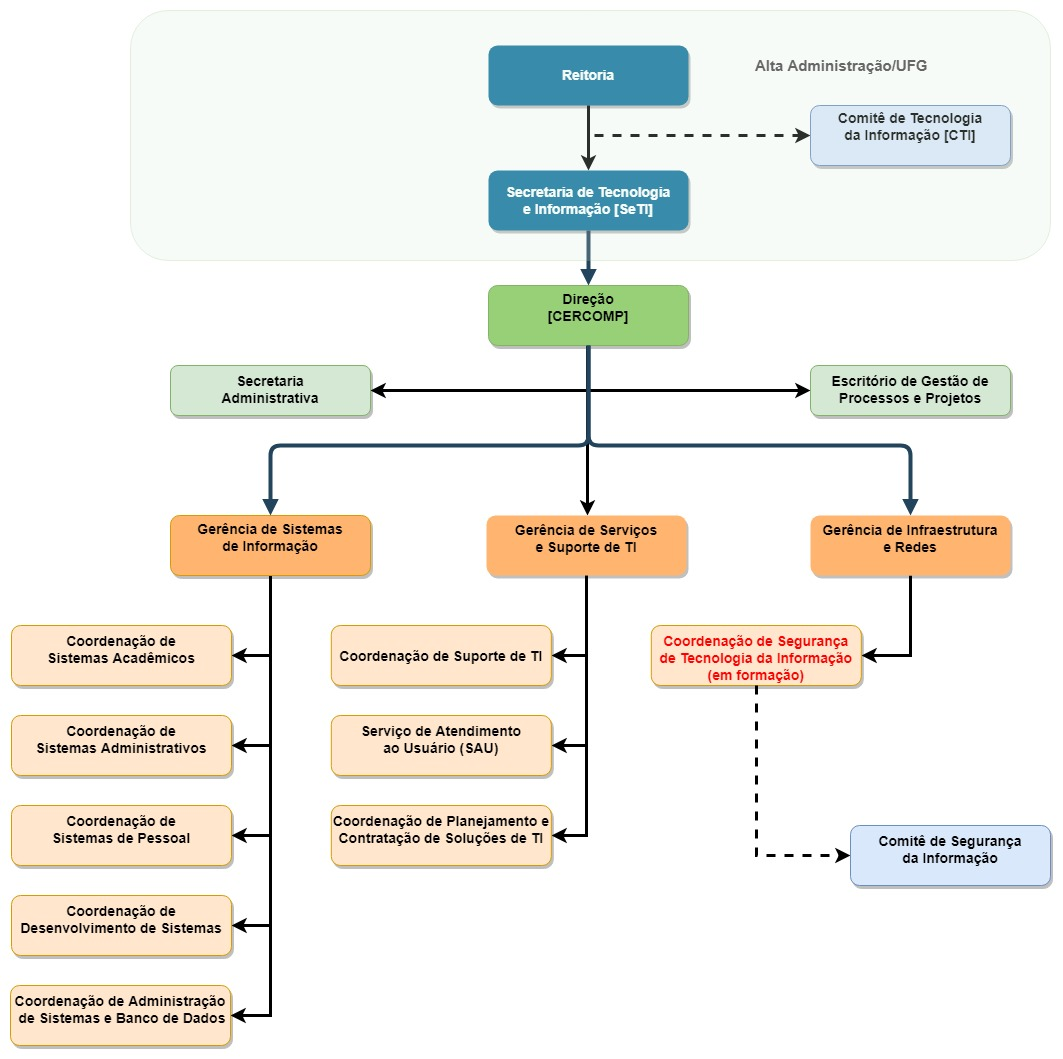
\includegraphics[width=1\textwidth]{./fig/organograma-cercomp-completo.jpg}
  \caption[Proposta de Organograma do CERCOMP.]{Proposta de Organograma do Cercomp.}
   \label{fig:organograma-cercomp}
\end{figure}

\section{Justificativa}
\label{sec:justificativa}

Durante sua trajetória, o CERCOMP foi incorporando e disponibilizando gradativamente à comunidade universitária da UFG diversos serviços de TI. Contudo, a disponibilização desses serviços não foi acompanhada de uma sistemática de processos para garantir sua especificação, divulgação e gestão de atendimento, tornando esses serviços, por algumas vezes, desconhecidos até entre as equipes técnicas do órgão.

Adicionalmente, a ferramenta de gerenciamento de serviços adotada pela instituição (GLPI) não possui integração com o Catálogo de Serviços de TI, até porque o mesmo é inexistente. Esse cenário prejudica o atendimento aos usuários e o gerenciamento dos serviços pela equipe técnica do órgão, de forma a comprometer a qualidade dos serviços prestados.

De maneira resumida, observa-se alguns problemas relacionados ao atendimento dos chamados de TI pelo CERCOMP: dificuldade, por parte da equipe do Serviço de Atendimento ao Usuário - SAU (\textit{helpdesk}), em identificar e direcionar determinados tipos de chamados; ausência de prazos definidos para atendimento ao usuário; indefinição e/ou desconhecimento do conjunto de serviços de TI ativos e disponíveis, entre outros.

Além das dificuldades observadas no encaminhamento e atendimento de solicitações de serviços de TI, há um outro fator tem se tornado determinante ao desenvolvimento de ações para o gerenciamento de serviços de TI do CERCOMP: o atendimento às exigências e determinações provenientes das atividades de fiscalização e acompanhamento dos ministérios e órgãos de controle.

Anualmente, as atividades de gestão da UFG são objeto auditorias de órgãos de controle tais como TCU (Tribunal de Contas da União) e CGU (Controladoria Geral da União). O Relato Integrado de Gestão UFG - 2018~\cite{RelatorioGestao2018}, apresentado junto à CGU, possui uma seção (Anexo G) dedicada à ``Gestão da tecnologia da informação da unidade jurisdicionada'', a qual tem por objetivo colher informações sobre a governança e gestão de TI, assim como dos serviços de TI oferecidos aos cidadãos.

A UFG, enquanto órgão da administração federal indireta, na condição de autarquia, integra o Sistema de Administração dos Recursos de Tecnologia da Informação (SISP) do atual Ministério da Economia. O SISP é um sistema (órgão central) instituído com o objetivo de gerir os recursos de TI da Administração Pública Federal Direta, Autárquica e Fundacional e, para tanto, estabelece um conjunto de diretrizes e normas a serem seguidas pelo órgãos vinculados.

A disponibilização do Catálogo de Serviços de TI também consta como meta do Plano Diretor de Tecnologia da Informação - PDTI/UFG (2018/2021 p.49)~\cite{PDTI2018} que, por sua vez, está alinhado ao Plano de Desenvolvimento Institucional - PDI/UFG (2018-2022 p.69)~\cite{PDI2018}. Isso demonstra o reconhecimento e interesse estratégico da Alta Administração e do CERCOMP sobre a sua necessidade e relevância dessa iniciativa para o aprimoramento do gerenciamento dos serviços de TI.

Dessa forma, mais do que uma necessidade entende-se que a disponibilização do Catálogo de Serviços de TI é uma oportunidade para  aprimorar a qualidade e centralizar em um único local as informações sobre os serviços de TI, de forma a atender tanto as diretrizes e exigências dos órgãos de controle quanto os objetivos e metas institucionais estabelecidos para a área de TI.


\section{Objetivos}
\label{sec:objetivos}

O objetivo geral deste trabalho é propor um modelo de referência para elaboração e gerenciamento do Catálogo de Serviços de TI, no âmbito da UFG, incluindo artefatos para especificação de serviços, acordo de nível de serviços e acordo de nível operacional, bem como definição de processos relacionados, de forma a contribuir para o aprimoramento dos serviços oferecidos pelo CERCOMP à comunidade universitária da UFG.

Por sua vez, os objetivos específicos são:
\begin{enumerate}
  \item Levantar e categorizar os serviços de TI oferecidos pelo CERCOMP à comunidade universitária, de forma a oferecer as condições necessárias para a elaboração, disponibilização e gerenciamento do Catálogo de Serviços de TI da UFG;
  \item Propor modelos para especificação de serviços, acordo de nível de serviços e acordo de nível operacional, determinando seus atributos e outras informações de interesse, e aplicando-os em um projeto técnico junto ao CERCOMP e, mais especificamente, à Equipe de Infraestrutura;
  \item Definir processos para elaboração, disponibilização e gerenciamento do Catálogo de Serviços de TI, bem como indicar modelos de documentos e ferramentas que possam apoiar as atividades;
  \item Avaliar e sugerir alternativas para o aprimoramento do Catálogo de Serviços de TI, considerando possibilidades de automatização e integração com a ferramenta de gerenciamento de serviços de TI adotada pela instituição.
\end{enumerate}


\section{Metodologia}
\label{sec:metodologia}

O presente trabalho constitui-se como um projeto técnico, o qual baseia-se nas melhores práticas disponíveis na literatura relacionadas ao gerenciamento dos serviços de TI, no intuito de propor um modelo de referência para elaboração e gerenciamento do Catálogo de Serviços de TI na UFG.

Para tanto, utilizou-se de revisão bibliográfica, análise diagnóstica, consulta e realização de webconferência com outras IFES para compartilhamento de experiências sob o tema, pesquisa exploratória na internet e a colaboração do Grupo de Trabalho (GT) do CERCOMP, responsável pela elaboração do Catálogo de Serviços de TI do órgão, de forma a diversificar a abordagem metodológica a ser aplicada no trabalho.

Conforme será apresentado no Capítulo~\ref{cap:estudo_caso}, para realização do projeto técnico optou-se por empregar uma abordagem contemplando o levantamento e categorização de todos os serviços externos oferecidos pelo CERCOMP à comunidade universitária da UFG e, após, aplicando modelos de documentos sugeridos em uma das categorias de serviços oferecidos pela Equipe de Infraestrutura do CERCOMP.


\section{Estrutura}
\label{sec:estrutura}

Para uma melhor compreensão de como este trabalho está organizado foi adotada a seguinte estrutura: o Capítulo~\ref{cap:introducao} é introdutório e apresenta o contexto, motivações e objetivos do trabalho.
Já no Capítulo~\ref{cap:conceitos} são apresentados os conceitos básicos e preliminares sobre o tema.
O Capítulo~\ref{cap:estudo_caso} demonstra o projeto técnico aplicado junto ao CERCOMP e, mais precisamente, à Equipe de Infraestrutura, sendo o mesmo organizado em três etapas.
Por fim, no Capítulo~\ref{cap:consideracoes_finais} são apresentadas as considerações finais e perspectivas de trabalhos futuros.
Na sequência, ainda compõem o trabalho as referências bibliográficas e os apêndices.
